\chapter{Asking Orlando Millionaires How They Got Rich}

We begin not with a theorem but with a promise. The lecture opens by throwing a few hard numbers at us---real estate, insurance and risk management, \(45{,}000\) apartment units, an \(\$11.5\) million deal, and a blurred admission of seven- or eight-figure earnings---and then it resets on the street in Orlando and Winter Park to ask how such outcomes are actually produced. There is no blackboard mathematics here, so the equations below are not transcriptions of written formulas; they are compact editorial renderings of mechanisms stated verbally in the interviews.

\section{Opening Montage and Field Reset}

The teaser montage should be read as compressed evidence, not as the lecture's first developed argument. It establishes the range of the field: multiple industries, several scales of operation, and a repeated concern with what turns work into wealth. Only after that does the lecture slow down and begin its inquiry in earnest: what industry did you choose, what was the largest deal, what was the biggest year, and what advice survives contact with the market?

\begin{table}[h]
\centering
\begin{tabular}{|l|l|}
\hline
Claim & Value \\
\hline
Apartment units managed & \(45{,}000\) \\
Largest real-estate deal mentioned & \(\$11.5\,\text{million}\) \\
Agency revenue last year & \(\$3\,\text{million}\) \\
Agency target this year & \(\$5\,\text{million}\) \\
Peak monthly income claim & \(\$75{,}000\) \\
Businesses previously owned & \(9\) \\
\hline
\end{tabular}
\caption{Selected quantitative claims made in the lecture. These are speaker claims, preserved as evidence rather than audited statements.}
\end{table}

\begin{remark}
The teaser's reference to ``seven or eight figures'' is imprecise and should remain a weak range claim only. We preserve the scale signal, but we do not sharpen it into a definite number.
\end{remark}

\section{From People Skills to Organizational Scale}

The first substantial case comes from the owner of a social media agency. The lecture does something important here: it begins with an origin that does not sound grand. The business ``kind of happened by accident,'' but it did not happen without structure. The owner emphasizes hustling, being good with people, and being able to operate comfortably around people much older than herself. In other words, the lecture begins with a reminder that commercial motion may start in social competence before it becomes managerial architecture.

The numbers then force the issue. Last year, the business did three million dollars in revenue, and the target for the coming year is five million. If we translate that verbal target into a simple growth calculation, we obtain
\begin{equation}
g_{\text{target}}
=
\frac{R_{\text{target}}-R_{\text{last}}}{R_{\text{last}}}
=
\frac{5-3}{3}
=
\frac{2}{3}
\approx 0.667.
\end{equation}
So the announced ambition is not a marginal improvement but roughly a \(66.7\%\) jump from the prior year. The lecture does not linger on this arithmetic, but it matters: the later discussion of leadership is not decorative advice; it is the organizational condition for sustaining that kind of increase.

\subsection{Question \& Answer}

\paragraph{Question.} What actually changes between a six-figure business and a seven-figure business?

\paragraph{Answer.} The lecture's answer is organizational rather than psychological. A six-figure business may still live inside the owner's direct control. A seven-figure business forces a transfer from personal effort to delegated throughput.

We may summarize the speaker's logic by introducing two editorial symbols:
\[
T_{\text{solo}} = \text{throughput under direct personal control},
\qquad
T_{\text{team}} = \text{throughput under delegated fulfillment}.
\]
The threshold claim is then
\begin{equation}
T_{\text{team}} > T_{\text{solo}}.
\end{equation}

The derivation is simple and worth stating explicitly:
\begin{enumerate}
\item A six-figure business can be run by one person who is ``the chief executive of everything.''
\item Once the business crosses into seven figures, the owner must train people, build a team, and tolerate the imperfect development of people who are ``almost there.''
\item Trust becomes part of production, because fulfillment for clients is now partly executed by others.
\item Therefore the scale variable is no longer only personal labor; it is the controlled expansion of organizational throughput.
\end{enumerate}

This is one of the lecture's recurring moves: a visible outcome is translated back into an invisible operating structure.

\section{Market Knowledge, Sales Discipline, and Equity}

The technology CEO sharpens the discussion. Here the lecture pivots away from hustle in general and toward commercial precision. The business is described concretely: a software platform for hospitality, with some extension into travel. But the lecture immediately refuses the naive moral that wealth in technology begins with technology itself.

\subsection{Question \& Answer}

\paragraph{Question.} Why can strong technology still fail to make money?

\paragraph{Answer.} Because, in the lecture's formulation, building is not selling. One may know the product and still not know the market; one may admire the technology and still fail to move a buyer.

A compact reconstruction of the sales logic is
\begin{align}
\text{market knowledge} &\Rightarrow \text{credible pitch}, \\
\text{credible pitch} &\Rightarrow \text{direct ask}, \\
\text{direct ask} &\Rightarrow \text{scheduled next step}.
\end{align}
Each arrow here condenses a sentence from the interview. Know the marketplace better than the technology. Research the customer before the approach. Believe in what you are selling, because uncertainty shows up in the pitch. Be direct, because decision-makers hear too much noise already. And when the conversation reaches the familiar ``we'll follow up,'' do not leave the next state undefined.

The most practical update rule in the lecture is therefore not an equation of price or probability, but a rule about state transition:
\begin{enumerate}
\item A promising meeting ends in verbal intent.
\item Verbal intent is unstable.
\item Immediate scheduling converts intent into a concrete next state.
\item Even if the meeting later moves, the relation remains structured rather than floating.
\end{enumerate}
This is why the lecture insists: book the appointment now.

From sales the lecture moves to ownership. Wealth is not described as salary maximization but as ownership of equity. A clean way to encode the underlying claim is
\begin{equation}
W_{\text{equity}} \propto \alpha V,
\end{equation}
where \(\alpha\) denotes an ownership share and \(V\) the value of the business. This is not a spoken equation, but it is exactly the structure behind the claim that if one does not have equity, one does not have wealth.

\begin{definition}
Sweat equity is ownership obtained through contribution, skill, and value brought to the firm rather than through founding status or initial cash investment.
\end{definition}

The same segment also introduces applied AI. The recommendation is not abstract futurism; it is operationally narrow. Find a simple utility that can be automated and license it. Later in the lecture, AI returns as an assistant-like layer that reduces routine burden. In the same editorial spirit we may write
\begin{equation}
t_{\text{ops}}\downarrow \Rightarrow E_{\text{throughput}}\uparrow,
\end{equation}
meaning that a reduction in routine operational load raises usable productive capacity.

\section{Hustle, Energy, and the Durability of a Business}

A lighter bridge follows: a former nightclub promoter now in the humanitarian space warns against the old life, describes very hard work, and complains that many aspiring entrepreneurs do not want to work at that level. The host then gives us a useful aside: interviews are sometimes initiated simply because someone has the look and the energy that make them worth approaching. This passage should not be overburdened with theory, but it does matter. It reminds us that the lecture is not a studio lecture pretending to be a walk; it is a live filtration of people in public.

The next major voice is more institutional. The operator in insurance, risk management, and academics supplies the lecture's most mature account of durability. Here the structure thickens: growth, retention, small excellences, and the double-edged character of people.

\subsection{Question \& Answer}

\paragraph{Question.} What makes a business look durable rather than fragile?

\paragraph{Answer.} The lecture gives three conditions. First, the business must grow, even if only a little. Second, it must keep good people long enough that outsiders can see continuity. Third, it must do small things well.

The growth condition may be formalized cautiously as
\begin{equation}
g = \frac{\Delta R}{R},
\qquad
g>0.
\end{equation}
The lecture does not define a precise accounting interval, but the sign is the point: investors do not want to fund shrinkage.

The people condition is stated with almost brutal symmetry. People are the greatest asset and the greatest liability. We may write, in a deliberately schematic way,
\begin{equation}
\text{good people} \Rightarrow \text{capability},
\qquad
\text{bad people} \Rightarrow \text{organizational damage}.
\end{equation}
This is immediately connected to retention. When a new hire meets colleagues who have been present for fourteen, ten, or nine years, the firm's continuity becomes legible without any slogan.

Finally, the lecture gives a sentence that deserves to survive intact in spirit: excellence is a lot of small things done well. That is why the old saying about tripping over molehills appears here. The point is not ornamental wisdom. It is a claim about error structure. Most businesses are not destroyed by one grand theorem failing; they are degraded by repeated local sloppiness.

The section closes with a compact theory of sales character. One must be uncommon without becoming weird; one must be respected before being persuasive. The lecture compresses the problem to a single buyer's question: why should I buy anything from you? We should preserve that compression in the final notes.

\section{Apprenticeship, Real Estate Discipline, and the Modern Wealth Stack}

The lecture then steps back into a more developmental register. We hear from someone who moved through marketing and sport and exercise science into life alignment coaching. The advice here is epistemic: know more, know that you know more, keep learning from others, accept help, and accumulate experience so that plateau is avoided. This matters because it prepares the transition to Trey and then to his grandfather. The lecture wants us to move from self-development into intergenerational apprenticeship.

Trey introduces his grandfather not as a myth but as a specific operator in commercial real estate around Winter Park and Park Avenue. The grandfather's own account is equally unsentimental. Real estate was not the dream. It was the vehicle. That distinction is crucial: the lecture repeatedly treats industry choice as an instrument and not as an identity badge.

\subsection{Question \& Answer}

\paragraph{Question.} How do we enter an industry we do not yet fully understand without pretending expertise?

\paragraph{Answer.} The lecture's answer is to enter as an apprentice to reality. Take the vehicle seriously, proceed in steps, copy successful operators, and refuse the seduction of over-leverage.

The anti-leverage doctrine is stated verbally, but its logic is cumulative:
\begin{enumerate}
\item Do not spend what you do not have to get what you do not need.
\item Avoid over-leverage, because financial stress degrades decision quality.
\item Start with the bottom step and move upward step by step.
\item Learn by imitation before improvisation: study successful people in the same market.
\end{enumerate}

The striking phrase is that wealth-building is a ``two point game,'' not a contest built on constant three-pointers. A natural reconstruction of that compounding idea is
\begin{equation}
W_n = W_0 \prod_{i=1}^{n} (1+r_i),
\end{equation}
where each \(r_i\) is a modest incremental gain rather than a miraculous leap. This is not the lecture's notation, but it captures exactly the speaker's insistence that repetition of manageable wins dominates the fantasy of sudden, repeated jackpots.

The lecture then moves to the closing real-estate specialist, and here several earlier lines of thought are gathered into one place: mentoring the inexperienced, using coaches and resources, high-quality service, referral-based selling, creator monetization, and AI.

The referral logic is explicit enough to merit a compact chain:
\begin{equation}
Q_{\text{service}}\uparrow
\Rightarrow
S_{\text{client}}\uparrow
\Rightarrow
R_{\text{referrals}}\uparrow
\Rightarrow
C_{\text{cold}}\downarrow.
\end{equation}
We may display the same structure as a transcript-backed schematic:

\begin{figure}[h]
\centering
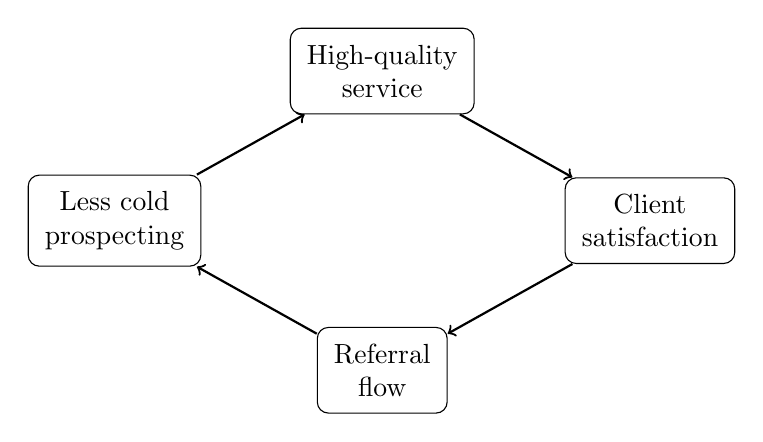
\begin{tikzpicture}[scale=1, every node/.style={draw, rounded corners, align=center, inner sep=6pt}]
\node (q) at (0,1.9) {High-quality\\service};
\node (s) at (3.4,0) {Client\\satisfaction};
\node (r) at (0,-1.9) {Referral\\flow};
\node (c) at (-3.4,0) {Less cold\\prospecting};
\draw[->, thick] (q) -- (s);
\draw[->, thick] (s) -- (r);
\draw[->, thick] (r) -- (c);
\draw[->, thick] (c) -- (q);
\end{tikzpicture}
\caption{Transcript-backed schematic of the referral flywheel described in the closing real-estate segment.}
\end{figure}

The creator discussion then adds a ranked monetization sequence. Attention is not yet a business. The lecture urges creators to treat brand deals as late, not early, revenue. A concise rendering is
\begin{equation}
M_{\text{affiliate}} \rightarrow M_{\text{owned}} \rightarrow M_{\text{brand}}.
\end{equation}
Affiliate revenue comes first, then owned products and services, and only then brand deals. The reason is strategic rather than moral: one should build something of one's own before renting out the attention one has captured.

The last move returns to AI. The lecture now treats AI less as an industry and more as a layer of business support. It can systemize work, simplify time and effort, and free attention for more valuable activity. This is the same operational logic we saw earlier in the software segment, but now widened to the contemporary wealth stack of real estate, creator business, and AI-supported services.

\section{Summary}

The lecture begins with spectacle and ends with operating rules. Across social media, software, insurance, nonprofit work, coaching, and real estate, the recurring lesson is that wealth is rarely explained by one dramatic insight alone. The mechanisms are steadier: organizational throughput beyond solo effort, knowledge of the market before devotion to the product, ownership rather than wages alone, growth that remains positive, careful handling of people, discipline against over-leverage, service that compounds into referrals, monetization that prioritizes owned value, and AI used as leverage rather than as ornament.

There is no blackboard here, but there is structure. If we keep the lecture in order, preserve the repeated questions, and translate only where the transcript genuinely supports translation, the resulting notes do not become thinner for lacking formal physics. They become a compact map of operational wealth-building.